\documentclass{beamer}
\usetheme{VATT}

\usepackage[utf8]{inputenc}
\usepackage[T1]{fontenc}
\usepackage{natbib}
\usepackage{hyperref}
\usepackage{multirow}

%% This presentation template builds on Gelugor Beamer theme developed by Lian Tze Lim
%% Use any fonts you like.
\usepackage{helvet}

\title{Puzzle}
\subtitle{Développement pour mobiles M1}
%\author{VATT Communication}
\author[Payet Jeremy]{
      Payet Jeremy  
}
\date{\today}

\begin{document}

\begin{frame}[plain,t]
\titlepage
\end{frame}

\section{Sommaire}
\begin{frame}
\frametitle{Sommaire}
\begin{itemize}
\item Introduction
	\begin{itemize}
	\item Quel est le projet ?
	\item Comment a-t-il été mis en place ?
	\end{itemize}
\item Détail du projet
\begin{itemize}
	\item Réalisation pour Android
	\item Réalisation pour iOS
	\end{itemize}
\item Conclusion
\end{itemize}
\end{frame}

\section{Introduction}
\subsection{Quel est le projet ?}
\begin{frame}
\frametitle{Quel est le projet ?}

Pour ce projet, nous avions différentes notions à implémenter dans une application de notre choix: 
\begin{itemize}
\item Changements de configuration
\item Internationalisation
\item Géolocalisation
\item Capteurs
\item Lecture audio
\item Gestes courants
\item Appareil photo
\end{itemize}

\end{frame}

\subsection{Comment a-t-il été mis en place ?}
\begin{frame}
\frametitle{Comment a-t-il été mis en place ?}
Comme il fallait implémenter tout ces éléments, il a fallu savoir à quoi peut servir chaque notion.Le changement de configuration et l'internationalisation ont été utilisé pour la langue et fixer au format portrait, les capteurs pour le mélange de puzzle en secouant l'appareil mobile, les gestes courants pour déplacer les images,et l'appareil photo pour créer l'image qui servira de puzzle. La géolocalisation a été considéré pour connaître l'origine des photos, mais n'a pas été implémenté
\end{frame}

\section{Détail du projet}
\subsection{Réalisation pour Android}

\begin{frame}
\frametitle{Réalisation pour Android}
\begin{center}
  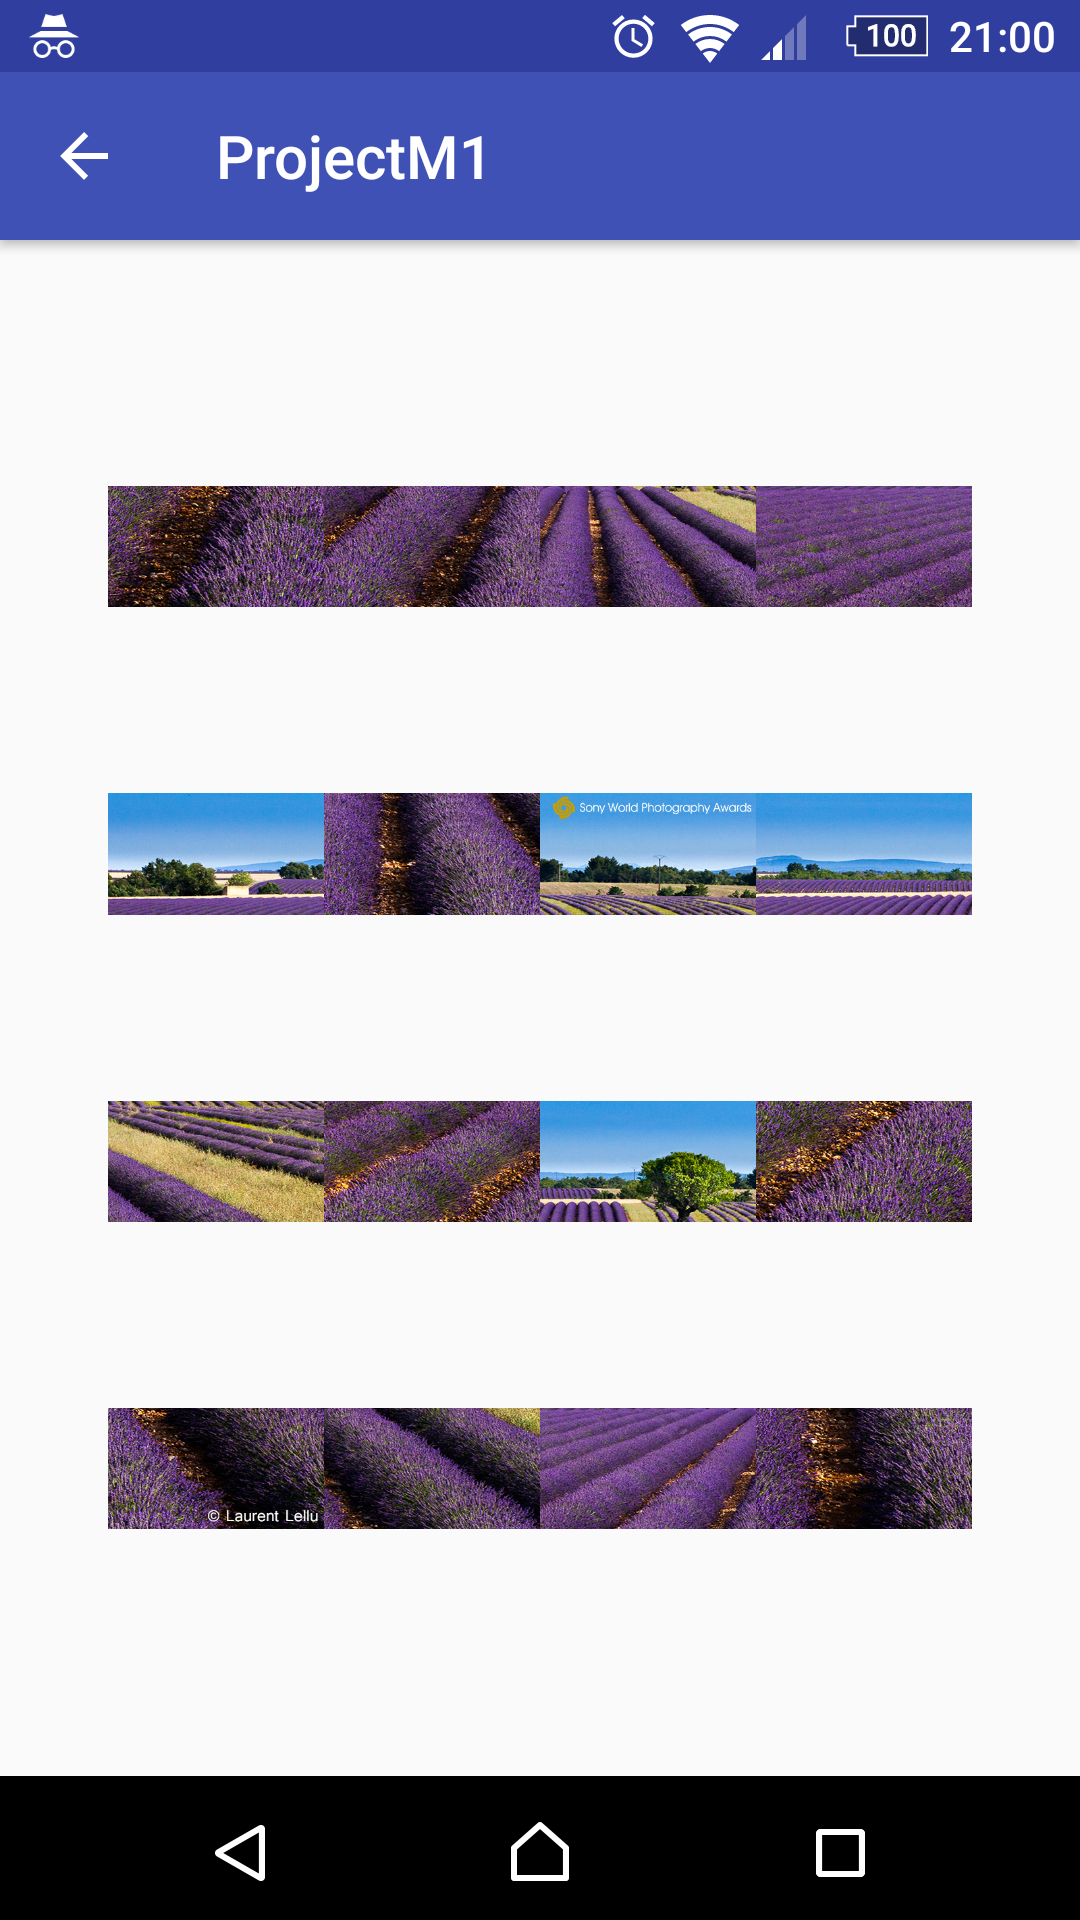
\includegraphics[scale=0.1]{android_menu.png}
\end{center}
\end{frame}

\begin{frame}
\frametitle{Réalisation pour Android}
\begin{center}
  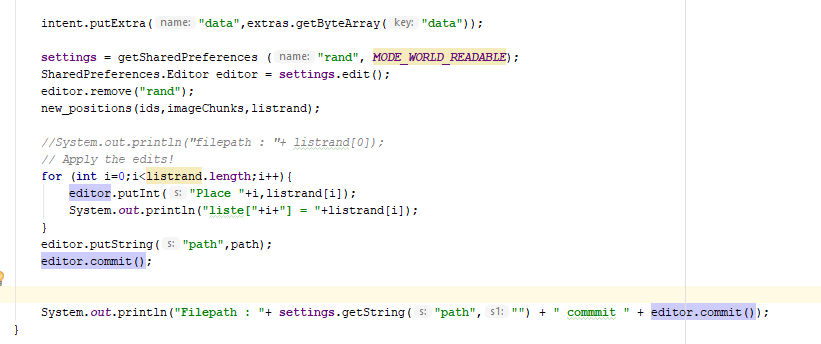
\includegraphics[scale=0.5]{JavaCode1.png}
\end{center}
\end{frame}

\subsection{Réalisation pour iOS}
\begin{frame}
\frametitle{Réalisation pour iOS}
\begin{center}
  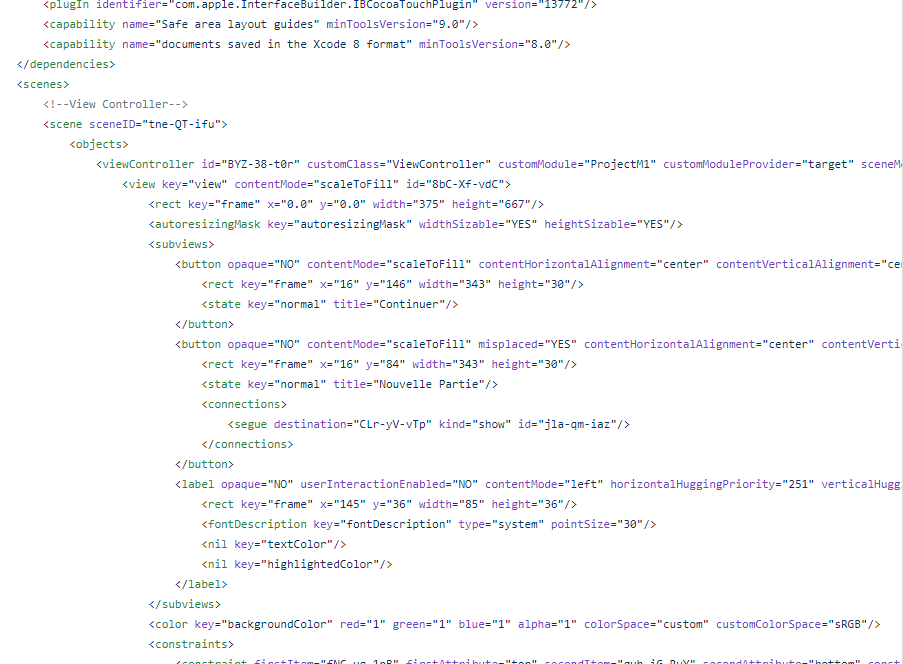
\includegraphics[scale=0.4]{ios_picture1.png}
\end{center}
\end{frame}

\begin{frame}
\begin{center}
  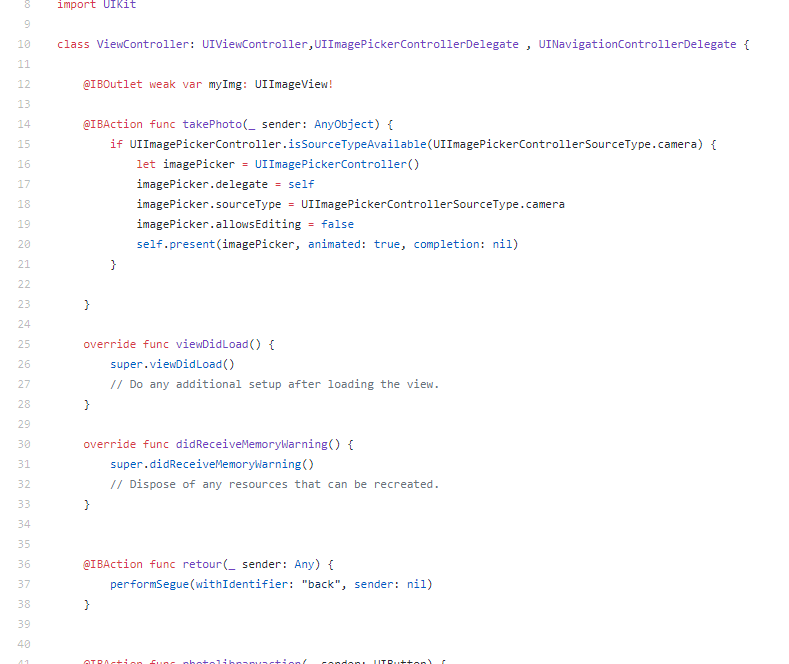
\includegraphics[scale=0.3]{iosCode1.png}
\end{center}
\end{frame}

\section{Conclusion}
\begin{frame}
\frametitle{Conclusion}
Au final, réaliser ce projet m'a posé des difficultés,surtout au niveau iOS. Les méthodes sous Android n'ont pas toutes été implémentés, même si elles ont été pensé.
\end{frame}

\end{document}